
\chapter{Bash statt SQL}
Um die Bash-Kommandos zu ersetzen, wird zuerst die Idee benötigt, wie sieht eine SQL-Anfrage in der Bash ausgedrückt mithilfe der klassischen Unix-Befehle aus, die textbasierte Datenbanken auslesen. Daher erklärt dieses Kapitel zuerst, wie Analysen auf Textdateien mit Kommandos wie cat, cut, awk und sed analog zu SQL-Abfragen aussehen. Anschließend werden damit Datenbank-Benchmarks implementiert und die Zeit der Abfragen bei großen Datenmengen gemessen. Der Vergleich mit neueren Programmen erfolgt dann im nächsten Kapitel.

\begin{figure}[htb]
\centering
Punktetabelle: \hspace{6cm} Zeittabelle:\\
\begin{tabular}{p{1cm}|p{3cm}|p{1cm}}
\hline
ID & Name & Punkte \\ \hline
1 & Franz & 50 \\ \hline
2 & Alfred & 10 \\\hline
3 & Marie & 27 \\\hline
\end{tabular}
\hspace{3cm}
\begin{tabular}{p{1cm}|p{1cm}}
\hline
ID & Zeit\\ \hline
1 & 44 \\ \hline
2 & 88 \\\hline
3 & 67 \\\hline
\end{tabular}
\caption{Beispiel Datenbank}
\label{fig:bspDB}
\end{figure}

\section{Relationale Algebra der Unix-Shell im Vergleich zu SQL}
Welche Strukturen eines Shell-Skripts sind in welche SQL-Anweisungen zu übersetzen? Um dies besser vergleichen zu können, werden im Folgenden Ausdrücke der relationalen Algebra als Befehle der Unix-Shell ausgedrückt und eine äquivalente Abfrage in SQL angegeben. Als Grundlage für die relationale Algebra dienen Operatoren aus dem Buch Datenbanksysteme \cite{Kemper} und in diesem Kapitel werden ausschließlich die grundlegenden Kommandos der Unix-Shell verwendet, heute auch bekannt als GNU core utilities \cite{Gulbins}.
\subsection{Grundlage}
Die Ausgabe einer Tabelle in SQL ist recht schlicht.
\begin{lstlisting}[language=SQL]
 SELECT * FROM Punktetabelle
\end{lstlisting}
Für die Ausgabe einer Textdatei in der Shell dienen Befehlen wie \textit{cat}, \textit{more}, \textit{less}, ... Sie finden sich häufig, wenn vorher Daten durchgepiped werden.
\begin{lstlisting}[language=Bash]
 cat Punktetabelle;
\end{lstlisting}
\subsection{Selektion}
Wenn jetzt Tupel ausgewählt werden, die ein Prädikat erfüllen sollen, dann ist dies eine Selektion und es sind zwei Fälle zu unterscheiden:
Äquivalenz: $\sigma_{ID=3}(Tabelle)$ oder Vergleich $\sigma_{ID<3}(Tabelle)$ oder in SQL:\\
\begin{lstlisting}[language=SQL]
 SELECT * FROM Punktetabelle WHERE ID=3;
 SELECT * FROM Punktetabelle WHERE ID<3
 SELECT * FROM Punktetabelle WHERE Name='Marie'
\end{lstlisting}

Die allgemeine Lösung nutzt \textit{awk}, mit dem alle Vergleichsfunktionen einer höheren Programmiersprache implementiert sind, hierbei sind die Felder durch \textit{\$1,...,\$n} bezeichnet, \textit{\$0} steht für alle Felder, die Option \textit{-F,} bezeichnet das Feldtrennzeichen (Delimiter), anschließend folgt ein Muster und der Befehl, der ausgeführt wird (\textit{' pattern \{CMD\}'}), in diesem Fall zuerst die Bedingung \textit{\$1==3} und der Befehl zur Ausgabe, \textit{print \$0} gibt alle Spalten aus (das \textit{SELECT *} der SQL).
\begin{lstlisting}[language=Bash]
$ awk -F, '$1==3 { print $0 }' Punktetabelle.csv
$ awk -F, '$1>3  { print $0 }' Punktetabelle.csv
$ awk -F, '$2="Marie" { print $0 }' Punktetabelle.csv
\end{lstlisting}

Andere grundlegende Kommandos funktionieren meist nur bei kompletter Äquivalenz, wie \textit{grep}, das in einer Datei nach allen Vorkommen der gewünschten Zeichenfolge sucht. Bei \textit{sed} kann auch auf Äquivalenz geprüft werden, dabei ist es aber von Vorteil, zumindest den vorderen und hinteren Spaltentrenner mit anzugeben, oder gar alle möglichen:
\begin{lstlisting}[language=Bash]
$ grep -r '3,.*' Punktetabelle.csv
$ grep -r 'Marie' Punktetabelle.csv
$ sed -nr '/3,.*/p' Punktetabelle.csv
$ sed -nr '/Marie/p' Punktetabelle.csv
\end{lstlisting}

\subsection{Projektion}
Wenn nun einzelne Spalten ausgewählt werden, so wird die Projektion benötigt:\\
{$\Pi_{Name,Punkte}(Punktetabelle)$}\\

oder in SQL:
\begin{lstlisting}[language=SQL]
 SELECT Name FROM Punktetabelle
\end{lstlisting}
Das klassische Unix-Kommando dazu ist \textit{cut}, das es mit Hilfe der Option \textit{-f} erlaubt, einzelne Felder zu extrahieren, Felder werden beginnend beim ersten durch Aufzählung mit Kommata bestimmt (1,3) und ganze Bereiche mit Bindestrich ausgewählt (1-3 entspricht Feldern eins bis drei), der Spaltentrenner wird durch die Option \textit{-d} mitgeteilt (Standard: Leerzeichen).
\begin{lstlisting}[language=Bash]
$ cut -f2,3 -d, Punktetabelle.csv
\end{lstlisting}
Die Kommandos \textit{awk} und \textit{sed} erlauben die Projektion auch, ersterer Befehl einfach mit \textit{print}, bei sed müssen explizit die Spaltentrenner angegeben werden:
\begin{lstlisting}[language=Bash]
$ awk -F, '{print $2,$3}' OFS=, Punktetabelle.csv
$ sed -nr 's/([^,]*),([^,]*),(.*)/\2\3/p'
\end{lstlisting}
\subsection{Vereinigung}
Die Vereinigung $\Pi_{ID}(Punktetabelle) \cup \Pi_{ID}(Zeittabelle)$ ist am einfachsten in der Unix-Shell zu realisieren, schließlich unterstützt fast jeder Befehl durch Eingabe mehrerer Dateien das Zusammenfügen dieser. Für das Zusammenfügen oder Konkatenieren drängt sich \textit{cat} (concatenate) geradezu auf, dadurch definiert sich doch dieser, einfach alle Dateien der Reihe nach auflisten:
\begin{lstlisting}[language=Bash]
$ cat datei1 datei2
\end{lstlisting}
Und schon sind sie vereinigt, analog das Beispiel der oben gezeigten Projektion:
\begin{lstlisting}[language=SQL]
 SELECT ID FROM Punktetabelle
 UNION
 SELECT ID FROM Zeittabelle
\end{lstlisting}
Das Beispiel erfordert vorher die Selektion, daher werden zwei anonyme Pipes verwendet, das sieht dann so aus:
\begin{lstlisting}
$ cat <(cut -f1 -d, Punktetabelle.csv) \
	<(cut -f1 -d, Zeittabelle.csv)
\end{lstlisting}

\subsection{Kreuzprodukt}
Will man in der Shell das Kreuzprodukt
$Punktetabelle \times Punktetabelle$
bilden, so geschieht das in SQL durch Auswahl mehrerer Tabellen:
\begin{lstlisting}[language=SQL]
 SELECT * FROM Punktetabelle, Punktetabelle
\end{lstlisting}
In der Shell hilft einem auch hier \textit{awk} weiter, diesmal mit Feldern. Zuerst werden alle Eingabezeilen (leeres Suchmuster) oder nur die gewünschten wie bisher durchgegangen und in dem Feld aufsteigend gespeichert. 
Anschließend, also im Schlussteil (bezeichnet durch END), kann mit den Feldern alles produziert werden, das Kreuzprodukt erfolgt durch die Ausgabe mit print in einer doppelten For-Schleife.
\begin{lstlisting}[language=Bash]
cat Punktetabelle | awk -F\| '
        {
		lines[i++]=$0
        }
        END{
                for (i in lines)
                  for (j in lines)
                    print lines[i], lines[j]
        }
' OFS=,
\end{lstlisting}
\subsection{Mengendifferenz}
Um alle Mengenoperationen der Algebra abzudecken, wird auch noch die Differenz benötigt, geschrieben als $R-S$, zum Beispiel ergibt $\Pi_{ID}(Punktetabelle) - \Pi_{ID}(Zeittabelle)$ diejenigen Tupel, zu denen kein passender Eintrag in der Zeittabelle einthalten ist.
\begin{lstlisting}[language=SQL]
 SELECT ID FROM Punktetabelle
 EXCEPT
 SELECT ID FROM Zeittabelle
\end{lstlisting}
In der Unix-Shell gibt der Befehl \textit{comm} die Zeilen in drei Spalten aus, zuerst die nur der ersten Datei (1), dann die nur der Zweiten (2) und dann die aus beiden (3), durch Angabe der Zahlen, können die Spalten unterdrückt werden. Für den Vergleich müssen die Dateien aber sortiert sein.
Analog zur Algebra entspricht folgender Befehl der Differenz:
\begin{lstlisting}[language=Bash]
$ comm -23 R S
\end{lstlisting}
Angewandt auf die Beispieltabellen:
\begin{lstlisting}[language=Bash]
$ comm -23 <(cut -f1 -d, Punktetabelle.csv | sort) \
		 <(cut -f1 -d, Zeittabelle.csv | sort)
\end{lstlisting}

\subsection{Umbennenung}
Um alle Ausdrücke der relationalen Algebra abzudecken, fehlt nun noch die Umbenennung der Tabelle $\rho_{t1}(Punktetabelle)$ und einzelner Spalten $\rho_{Nr \leftarrow ID}(Punktetabelle)$. Da in der Shell die Tabellen nichts anders als Datenströme sind, ist keine Unterscheidung der Namen notwendig, eine Möglichkeit, die Tabellen umzubenennen, besteht nur darin, eine temporäre Hilfstabelle mit neuem Namen anzulegen.
\begin{lstlisting}[language=Bash]
$ cp Punktetabelle.csv t1.csv
\end{lstlisting}
Auch einzelne Spalten können nur mit ihrer Nummer angesprochen werden (\$1,\$2, etc.), eine Umbenennung kann nur für die Ausgabe erfolgen, der Strom muss also vorher mit \textit{awk} oder \textit{sed} bearbeitet werden.
\begin{lstlisting}[language=Bash]
$ sed -r 's/ID/Nr/' Punktetabelle.csv 
NR,Name,Punkte
1,Franz,50
2,Alfred,10
3,Marie,2
$ cat Punktetabelle | awk -F\| '
        NR==1{
		print "Nr", $2, $3
        }
        NR>2{
		print $0
	}
' OFS=,
\end{lstlisting}

\subsection{Relationaler Verbund}
Alle grundlegenden Operatoren der relationalen Algebra können auch mit einfachen Skripten auf textbasierten Datenbanken erfolgen, dennoch darf ein wichtiger Operator nicht fehlen, der relationale Verbund (Join), vor allem der natürliche Verbund (natural join), der Tabellen über Äquivalenz zusammengehöriger Attribute verknüpft:\\

$R \Join S $ 

oder im Beispielfall mit Verknüpfung über ID: $ Punktetabelle \Join Zeittabelle$\\
Der analoge Fall in SQL:
\begin{lstlisting}[language=SQL]
 SELECT *
 FROM Punktetabelle, Zeittabelle
 WHERE Punktetabelle.ID = Zeittabelle.ID
\end{lstlisting}

In Unix stehen für Equijoins jeglicher Art, bei denen jeweils ein Feld jeder Tabelle übereinstimmen soll, das Kommando \textit{join} zur Verfügung. Sollen zwei CSV-Dateien miteinander verknüpft werden, so müssen das Spaltentrennzeichen und die zu verknüpfenden Spalten (\textit{-1 spalteA -2 spalteB}) angegeben werden, standardmäßig der Leerraum (Whitespace) sowie die jeweils erste Spalte, und, sofern die erste Zeile die Bezeichner enthält, müssen diese als solche mit \textit{--header} deklariert sein.
\begin{lstlisting}[language=Bash]
$ join --header -t, -1 1 -2 1 Punktetabelle.csv Zeittabelle.csv
\end{lstlisting}
Zu beachten ist, dass im Ergebnis eine der verbundenen Spalten dann fehlt, also oben stehende Abfrage produziert folgendes Ergebnis:\\

\hspace{3cm}
\begin{tabular}{p{1cm}|p{3cm}|p{1.2cm}|p{1cm}}
\hline
ID & Name & Punkte & Zeit	 \\ \hline
1 & Franz & 50 & 44       \\ \hline
2 & Alfred & 10  & 88       \\\hline
3 & Marie & 27 & 67       \\\hline
\end{tabular}
\\\\
Die auszugebenden Spalten können auch hinter der Option \textit{-o} explizit angegeben werden, \textit{0} ist die verbundene Spalte, alle anderen mit der Spaltenummer der jeweiligen Tabelle, \textit{2.3} meint die dritte Spalte der zweiten Tabelle.
Also sollen die Spalten, für die die Join-Bedingung gilt, angezeigt werden und die zweite und dritte, so hilft folgender Befehl:
\begin{lstlisting}[language=Bash]
$ join -t, -o 0 1.2 1.3 tabelleA tabelleB
\end{lstlisting}
Damit können auch Semi-Joins $ R \ltimes S $ und $ R \rtimes S $ produziert werden, indem die Spalten angegeben sind, für einen linken Semi-Join sind das \textit{-o 1.1 1.2 \dots 1.n} und  für den rechten \textit{-o 2.1 2.2 \dots}\\

Ein Join der Shell ist ein Sort-Join, er funktioniert (wie \textit{comm} auch) nur auf sortierten Dateien, folglich muss oft eine Sortierung mit \textit{sort} erfolgen, bevor gejoint werden kann. Das Kommando \textit{sort} arbeitet mit Quicksort \cite{Prince}, also mit Durchschnittslaufzeit $O(n\ log\ n)$, in schlechten Fällen auch $O(n^2)$. Dabei muss der Sortierfunktion noch das Trennzeichen (\textit{-t,}) sowie die zu sortierenden Spalten als Feld angegeben werden, also \textit{-k2,3} sortiert nach dem zweiten und dritten Feld. Erfolgt ein Join danach, so ist zu empfehlen, nach exakt einer Spalte zu sortieren \textit{-k2,2}, da das Ergebnis sonst von der Länge des nachfolgenden Textes abhängt. 
\begin{lstlisting}[language=Bash]
$ sort -t, -k2,2 tabelleA | join -1 2 - tabelleB
\end{lstlisting}
\textit{sort} sortiert aber auch die Kopfzeile mit, also muss diese separat behandelt werden, am besten wird die erste Zeile mit \textit{head} extrahiert, alle anderen mit \textit{tail} und nach dem Sortieren können die Zeilen wieder zusammengefügt werden.
\begin{lstlisting}$
$ head -1 tabelleA > nurKopf
$ tail -n+2 tabelleA | sort -t, -k1,1 | cat nurKopf - > tabAmod
$ head -1 tabelleB > nurKopf2
$ tail -n+2 tabelleB | sort -t, -k1,1 | cat nurKopf2 - |\
  join -t, -1 1 -2 1 tabAmod - 
\end{lstlisting}

%Outer join äußerer Join (links und recht und alles), Antijoin
%
Auch der Antijoin $ R \vartriangleright S $ bzw. $ R \vartriangleright S$ ist in der Unix-Shell mit der Option \textit{-v1} und \textit{-v2} implementiert, der die Zeilen der ersten Tabelle (bzw. der zweiten) ausgibt, zu denen kein Partner in der anderen Tabelle gefunden wurde. Damit nur die benötigten Spalten ausgegeben werden, empfiehlt es sich, die Spalten mit der Option \textit{-o} noch explizit anzugeben:
\begin{lstlisting}[language=Bash]
$ join -t, -1 1 -2 1 -v1 -o 0 1.2 1.3 R.csv S.csv
\end{lstlisting}
Wenn zum Beispiel die Namen ausgegeben werden sollen, zu denen keine Zeit gemessen wurde, sieht das so aus:
\begin{lstlisting}
$ join -t, -1 1 -2 1 -v1 -o 1.2 Punktetabelle.csv Zeittabelle.csv
\end{lstlisting}

Als einzige Join-Arten, die noch fehlen, verbleiben die äußeren Joins
$R {\tiny \textifsym{d|><|d}} S $,
$R {\tiny \textifsym{d|><|}} S $ und
$R {\tiny \textifsym{|><|d}} S $,
die auch der Unix-Befehl mit der Option \textit{-a1} und \textit{-a2} erzeugt, wodurch alle Zeilen der ersten (analog der zweiten) Datei ausgegeben werden, auch solche mit fehlendem Join-Partner. Die fehlenden Werte, bei SQL die Null-Werte, können mit \textit{-e "Wert"} angegeben werden, sollen sie mit "'0"' aufgefüllt werden, dann mit \textit{-e "0"}.

\begin{lstlisting}[language=Bash]
$ join -t, -a1 -a2 -1 2 -2 2 -o 0 1.1 2.1 -e "0" tabelleR tabelleS
$ join -t, -a1     -1 2 -2 2 -o 0 1.1 -e "0" tabelleR tabelleS
$ join -t,     -a2 -1 2 -2 2 -o 0 2.1 -e "0" tabelleR tabelleS
\end{lstlisting}

\subsection{Gruppierung und Aggregation}
Über die relationale Algebra hinaus, geht der Gamma-Operator, der die Werte gruppiert und Aggregatsfunktionen wie max, min, sum oder avg auf ihnen erlaubt.
So gibt\\
$\gamma_{count(*)}(Punktetabelle)$
die Anzahl aller Teilnehmer aus. Aus dem Standard-Reportoire der Unix-Shell ist auch der Befehl \textit{awk} nützlich: Dazu sollten die Dateien vorher nach den Feldern sortiert sein, der Trick nutzt die Sortierung aus, die Werte der Spalten, nach denen gruppiert wird, wird vermerkt, die Aggregierung beginnt. Sobald sich ein Wert verändert, ist also zur nächsten Gruppe gesprungen worden, die aggregierten werden ausgegeben, die nächste Gruppe folgt, bis schließlich keine Zeilen mehr nachkommen, im END-Teil werden die letzten Aggregate ausgegeben.

\begin{lstlisting}[language=SQL]
SELECT spalte2, spalte3,
	max(spalte4), min(spalte4), count(*), avg(spalte4)
FROM Tabelle
GROUP BY spalte2, spalte3
\end{lstlisting}

Eine Gruppierung in \textit{awk} benutzt temporäre Variablen für die Summe, die Anzahl, das Minimun und das Maximum, der Durchschnitt setzt sich später aus Summe und Anzahl zusammen.
Zudem werden die Werte gespeichert, nach denen gruppiert wird. Ändern sich diese nicht, so werden die Werte der aktuellen Zeile in der Aggregation ergänzt, \textit{count} wird inkrementiert, der entsprechende Wert zur Summe von \textit{sum} addiert und nach größer und kleiner für \textit{min} und \textit{max} geschaut. Passen die Werte zum Gruppieren nicht überein, so werden die alten ausgegeben und die Aggregationsvariablen zurückgesetzt.

\begin{lstlisting}[language=Bash]
head -1 tmp.csv > tmp1.csv
tail -n+2 tmp.csv  | sort -t\| -k2,2 | cat tmp1.csv - | awk -F\| '
        NR==1{print $2, $3,
		"max(S4)", "min(S4)", "count(*)", "avg(S4)"
	}
        NR==2{g2=$2; g3=$3; count=1; max4=$4; min4=$4; sum4=$4}
        NR>2{
                if( g2==$2 && g3==$3 ){
                        count++; sum4+=$4;
			if(max4<$4)
				max4=$4;
			if(min4>$4)
				min4=$4;
                }else{
                        print g2,g3,
				max4,min4,sum4,count,sum4/count;
                        g2=$2; g3=$3;
			count=1; max4=$4; min4=$4; sum4=$4
                }
        }
        END{print g2,g3,max4,min4,sum4,count,sum4/count}
' OFS=\|
\end{lstlisting}

Eine einfachere Lösung bietet der Befehl \textit{uniq -c}, sofern nur die Anzahl der Vorkommnisse gezählt werden soll.

\section{Performanzmessungen}
Das vorherige Kapitel hat die Grundlagen erklärt, also wie die relationale Algebra, auf der die relationale Anfragesprache SQL basiert, auf textbasierte Datensätze angewandt werden kann. Dieses Kapitel behandelt die Performanz solcher Abfragen, also wie schnell sie sich ausführen lassen, auch im Vergleich zu modernen relationalen Datenbanken.

\subsection{TPC-H Benchmarks}
Um die Leistungsfähigkeit von Datenbanken zu testen, wurde im Jahr 1988 auf Initiative von Omri Serlin hin ein Konsortium namens Transaction Processing Performance Council (TPC) gegründet, an dem acht Firmen der IT-Branche beteiligt waren \cite{HistoryTPC}.
Das Ziel war es nicht, "`die Funktionen und Operationen von Rechnern zu testen, [sondern] Transaktionen zu betrachten, wie sie allgemein in der Geschäftswelt üblich sind: Der Tausch von Gütern, Dienstleistungen und Geld"' \cite{AboutTPC}.
So wurde der erste Benchmark für Datenbanksysteme entwickelt, genannt TPC-A, der die maximalen Transaktionen pro Sekunde misst, wenn von verschiedenen Endgeräten darauf zugegriffen wird. Der Anwendungsbereich der TPC-A Benchmark ist die Online-Verarbeitung von Transaktionen, \textit{Online Transaction Processing} (OLTP), wie sie in potentiellen Handelsunternehmen vorkommen, die Güter und Dienstleistungen gegen Geld tauschen. Sie "`[zeichnen sich aus] durch relativ kurze Transaktionen, die im Allgemeinen nur auf ein eng begrenztes Datenvolumen zugreifen."'\cite[S. 711]{Kemper}

Der aktuellste Standard für ad-hoc OLAP-Anwendungen ist der TPC-H Benchmark, der die Leistung der Datenbank bei analytischen Anfragen (ad-hoc analytical queries) misst, ohne dass die Datenbank zuvor darauf vorbereitet wird. Dazu sind 22 verschiedene Anfragen gegeben und eine Datenbasis, die mittels eines gegebenen Zufallsgenerators generiert wird, aber sich immer nach dem Handelsunternehmensschema aus acht Relationen richtet (vgl. Abb. \ref{fig:TPC-H-Schema}).

\begin{figure}
\centering
\includegraphics[scale=.6]{TPC-H-Schema}
\caption{TPC-H Schema \cite{TPC-H}}
\label{fig:TPC-H-Schema}
\end{figure}

Der Generator \textit{DBGen} erzeugt die Datenbasis in verschiedenen Größen mit unterschiedlich vielen Tupeln in Abhängigkeit eines Faktors \textit{SF}, der ungefähr der Größe aller Daten in GB entspricht, \textit{SF=1} steht für 1\ GB, die möglichen Größen sind 1\ GB, 10\ GB, 30\ GB, 100\ GB, 300\ GB, 1\ 000\ GB, 3\ 000\ GB, 1\ 0000\ GB, 30\ 000\ GB und 100\ 000\ GB an Daten, die per Zufall erstellt werden.

\begin{figure}[htb]
\centering
\begin{tabular}{p{2,5cm}|p{2,5cm}|p{2,5cm}|p{2,5cm}}
Table Name & Cardinality &  Length (in bytes) &  Typical Table \\\hline
SUPPLIER & 10,000  & 159&  2\\
PART 	& 200,000 &155& 30 \\
PARTSUPP & 800,000 & 144 & 110 \\
CUSTOMER & 150,000 & 179 & 26 \\
ORDERS   & 1,500,000 & 104 & 149 \\
LINEITEM &  6,001,215 & 112 & 641 \\
NATION & 25 & 128 & <1 \\
REGION & 5 & 124 & <1 \\\hline
Total & 8,661,245 && 956
\end{tabular}
\caption{Größe der Relationen bei Faktor SF=1 \cite{TPC-H}}
\end{figure}

\subsection{Implementierung mit Shell-Skripten}
Um nun die Leistungsfähigkeit der Shell-Skripte auf textbasierten Datenbanken zu testen, braucht es drei Werkzeuge: die Daten, die Skripte und natürlich Referenzwerte - die Skripte werden von Hand erzeugt, die Grundlage für die Datenbasis ist dieselbe wie für den TPC-H-Benchmark der Hyper-Schnittstelle\footnote{\url{http://hyper-db.de/interface.html}}, so lassen sich die Ergebnisse auch gut vergleichen.\\

Die Implementierung der SQL-Anfragen orientiert sich an dem vorgestellten Schema im letzten Unterkapitel, nachfolgend sei nur die vierte TPC-H-Anfrage vorgestellt, die Implementierungen der anderen erfolgen analog und sind im Anhang einzusehen. Die vierte Abfrage der Benchmark bewirkt Folgendes:

\begin{quotation}
"`Mit Hilfe dieser Anfrage soll überprüft werden, wie gut das Auftragsprioritätensystem funktioniert. Zusätzlich liefert sie eine Einschätzung über die Zufriedenstellung der Kunden. Dazu zählt die Anfrage die Aufträge im dritten Quartal 1993, bei denen wenigstens eine Auftragsposition nach dem zugesagten Liefertermin zugestellt wurde. Die Ausgabeliste soll die Anzahl dieser Aufträge je Priorität sortiert in aufsteigender Reihenfolge enthalten."' \cite[S. 717]{Kemper}
\end{quotation}


In SQL ausgedrückt sieht das so aus:

\begin{lstlisting}[language=SQL]
select
        o_orderpriority,
        count(*) as order_count
from
        orders
where
        o_orderdate >= date '1993-07-01'
        and o_orderdate < date '1993-10-01'
        and exists (
                select
                        *
                from
                        lineitem
                where
                        l_orderkey = o_orderkey
                        and l_commitdate < l_receiptdate
        )
group by
        o_orderpriority
order by
        o_orderpriority
\end{lstlisting}

Um die Anfragen in Skripte zu übersetzen, hilft die Orientierung am Abfrageplan (siehe Abb. \ref{fig:Queryplan4}). So erhält man einerseits den Ausdruck der relationalen Algebra dafür und eine Schritt-für-Schritt-Übersetzung ist möglich. Außerdem sind so die Ergebnisse besser vergleichbar. Die Tabellen liegen als CSV-Dateien mit Trennzeichen '|' in <tabellenname>.tbl vor, die Kopfzeilen analog in <tabellenname>.csv.

In diesem Fall müssen zuerst die Tabelle \textit{orders} und \textit{lineitem} nach den entsprechenden Tupeln gefiltert werden (o\_orderdate >= date '1993-07-01' and o\_orderdate < date '1993-10-01' und l\_commitdate < l\_receiptdate), in der Shell geschieht dies durch Auswahl der Zeilen mittels \textit{awk}.

\begin{lstlisting}[language=Bash]
sort -k1,1 -t\| orders.tbl | cat orders.csv - | awk -F\| '
        NR==1 || $5<"1993-10-01" && $5>="1993-07-01"{
                print $1"|" $6
        }
' > tmporder.csv

sort -k1,1 -t\| lineitem.tbl |cat lineitem.csv - | awk -F\| '
        NR==1 || $12<$13{
                print $1
        }
' | uniq  |\
\end{lstlisting}

Das anschließende \textit{exists} in SQL wird durch einen linken äußeren Join verwirklicht. Im Gegensatz zu einem Join soll nur auf Existenz überprüft werden, deshalb hilft das Unix-Kommando \textit{uniq} aus, um Duplikate zu eliminieren. 

\begin{lstlisting}[language=Bash]
join --header -t\| -1 1 -2 1 tmporder.csv - > tmp.csv
\end{lstlisting}

Im nächsten Schritt folgt die Gruppierung (\textit{group by}) auf die Spalte \textit{o\_orderpriority}, die einfach durch \textit{uniq} erfolgen kann, bei komplizierteren Aggregatsfunktionen (min, max, sum, count) ist es oft einfacher mit \textit{awk} zu hantieren.

\begin{lstlisting}[language=Bash]
head -1 tmp.csv > tmp1.csv
tail -n+2 tmp.csv  | sort -t\| -k2,2 | cat tmp1.csv - | awk -F\| '
        NR==1{print $2,"order_count"}
        NR==2{g2=$2; count=1}
        NR>2{
                if( g2==$2 ){
                        count++
                }else{
                        print g2, count;
                        g2=$2;count=1;
                }
        }
        END{print g2,count}
' OFS=\|
\end{lstlisting}

Für den Fall der vierten TPC-H-Abfrage kann aber auch \textit{uniq -c} benutzt werden, der neben der Gruppierung auch die Anzahl der Vorkommnisse aller Tupel mit ausgibt, dafür müssen wir uns zunächst auf die relevanten Spalten beschränken (mit \textit{cut}) und alle Zeilen auch sortieren, damit der letztere Befehl ordentlich funktioniert.

\begin{lstlisting}[language=Bash]
cut -d\| -f2 | tail -n+2 | sort | uniq -c
\end{lstlisting}

Und schon ist das Skript fertig, beide Versionen liefern die gewünschte Ausgabe:\\

{\centering \parbox{7cm}{
o\_orderpriority|order\_count\\
1-URGENT|10594\\
2-HIGH|10476\\
3-MEDIUM|10410\\
4-NOT SPECIFIED|10556\\
5-LOW|10487\\
}}
{\parbox{7cm}{
10594 1-URGENT\\
10476 2-HIGH\\
10410 3-MEDIUM\\
10556 4-NOT SPECIFIED\\
10487 5-LOW\\
}}

Die Implementierung aller weiteren TPC-H-Abfragen erfolgte analog. Die Abfragen wurden bei SF=1 und SF=10 getestet. Diese und alle nachfolgenden Läufe wurden auf einem Intel Core i7-3517U mit zwei Kernen (1.90GHz) getestet, die Läufe bei SF=10 erfolgten auf ScyPer-15 mit 40 Kernen.

\begin{figure}[h]
%\includegraphics[scale=.6]{Queryplan4}
\Tree [.sort [.$\gamma_{\$2, count(*)}$ [.$\ltimes_{orders.\$1=lineitem.\$1}$
[.$\sigma_{\$5<1993-10-01 \wedge \$5>=1993-07-01}$ orders ]
[.$\sigma_{\$12<\$13}$ lineitem ]
] ] ]
\caption{Abfrageplan zu Nummer 4}
\label{fig:Queryplan4}
\end{figure}

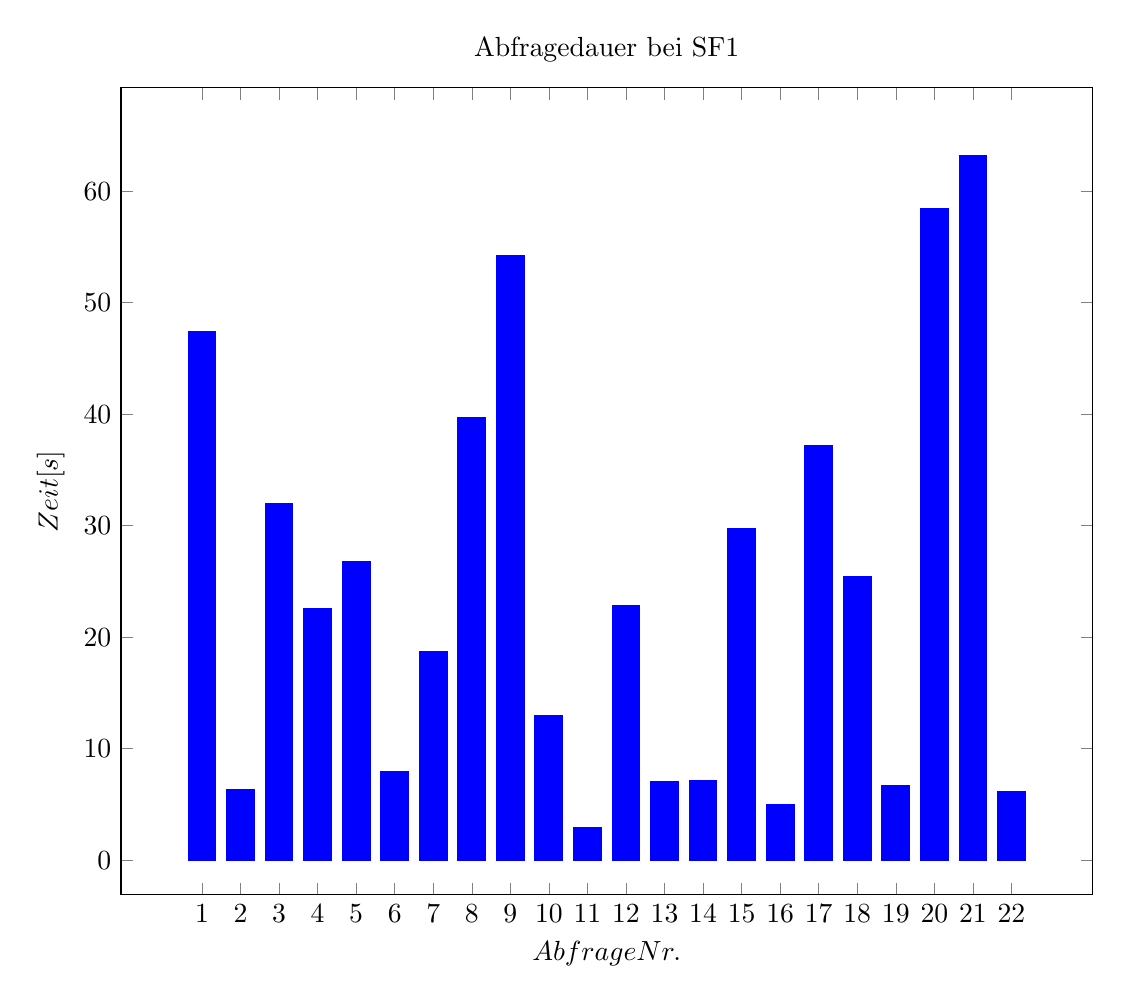
\begin{tikzpicture}
\begin{axis}[
xtick=data,
title=Abfragedauer bei SF1,
scale=1.8,
xlabel={$Abfrage Nr.$},
ylabel={$Zeit [s]$},
]
\addplot[
ybar,
fill = blue,
color = blue
] coordinates {
(1,47.420)
(2,6.372)
(3,32.022)
(4,22.544)
(5,26.827)
(6,7.949)
(7,18.713)
(8,39.677)
(9,54.243)
(10,12.971)
(11,2.934)
(12,22.859)
(13,7.068)
(14,7.185)
(15,29.784)
(16,4.957)
(17,37.156)
(18,25.484)
(19,6.728)
(20,58.405)
(21,63.225)
(22,6.178)
};

%\addplot[
%color=green,
%mark = *,
%only marks
%] coordinates{
%(3,29.276)
%(5,24.441)
%(7,17.680)
%(9,46.270)
%};
%\legend{nach Abfrageplan, Bash-optimierter Abfrageplan}
\end{axis}
\end{tikzpicture}

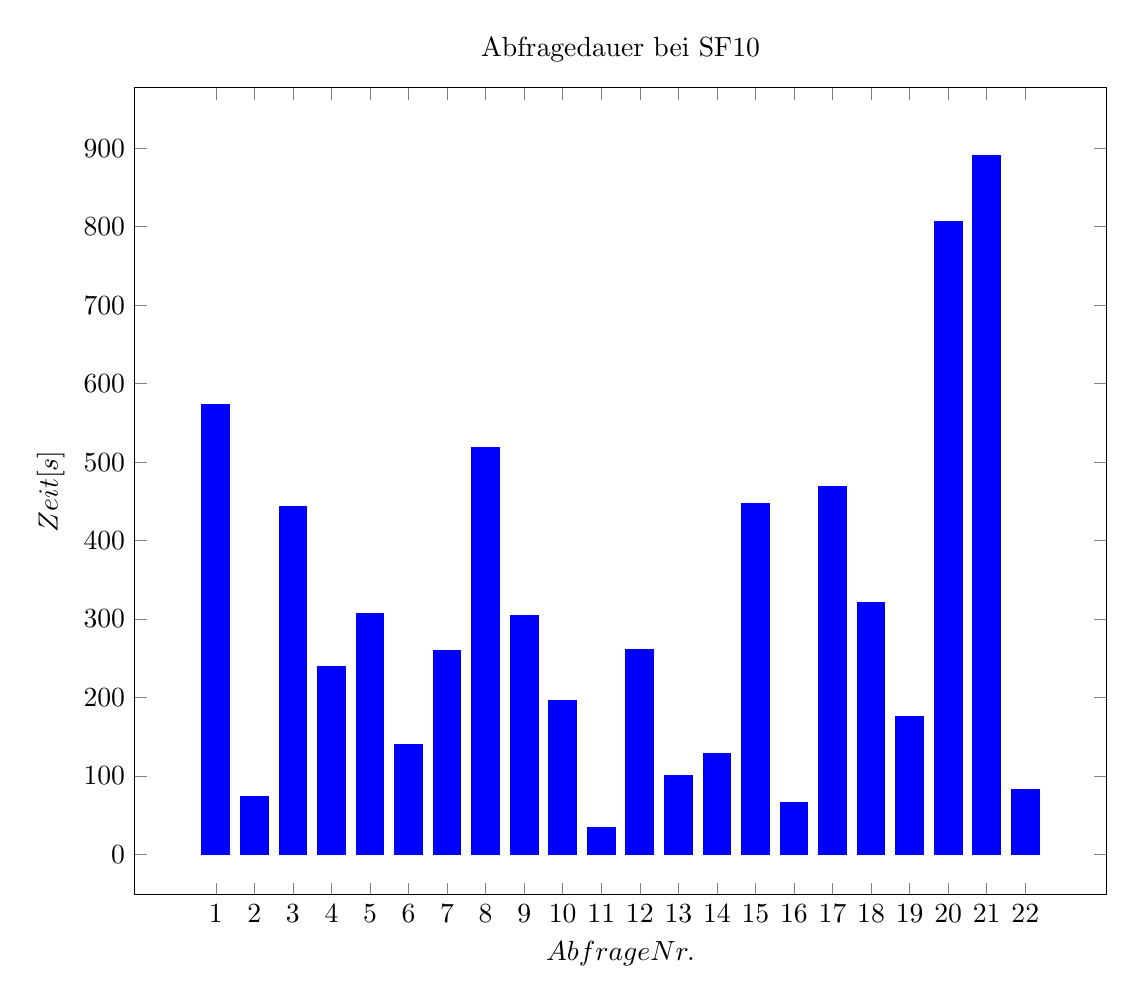
\begin{tikzpicture}
\begin{axis}[
xtick=data,
title=Abfragedauer bei SF10,
scale=1.8,
xlabel={$Abfrage Nr.$},
ylabel={$Zeit [s]$},
]
\addplot[
ybar,
fill = blue,
color = blue
] coordinates {
(1,	572.857)
(2,	73.534)
(3,	443.247)
(4,	234.677)
(4,	238.975)
(5,	307.112)
(6,	140.614)
(7,	260.438)
(8,	518.944)
(9,	304.204)
(10,	195.974)
(11,	34.194)
(12,	261.685)
(13,	100.206)
(14,	128.932)
(15,	446.731)
(16,	66.396)
(17,	468.63)
(18,	320.389)
(19,	175.907)
(20,	806.291)
(21,	891.314)
(22,	82.748)
};
\end{axis}
\end{tikzpicture}

\subsection{Optimierung durch Parallelisierung}
Ein kurzer Blick auf die laufenden Prozesse bestätigt einen Verdacht: die Abfragen laufen teils parallel, es werden so viele Prozesse gestartet wie Kommandos in einer Pipeline verwendet. Von den meisten heutigen Bash-Philosophen wird dies verschwiegen, daher lohnt sich ein Blick in das Buch von Pike und des awk-Erfinders Kernighan.

\begin{figure}[h]
\centering
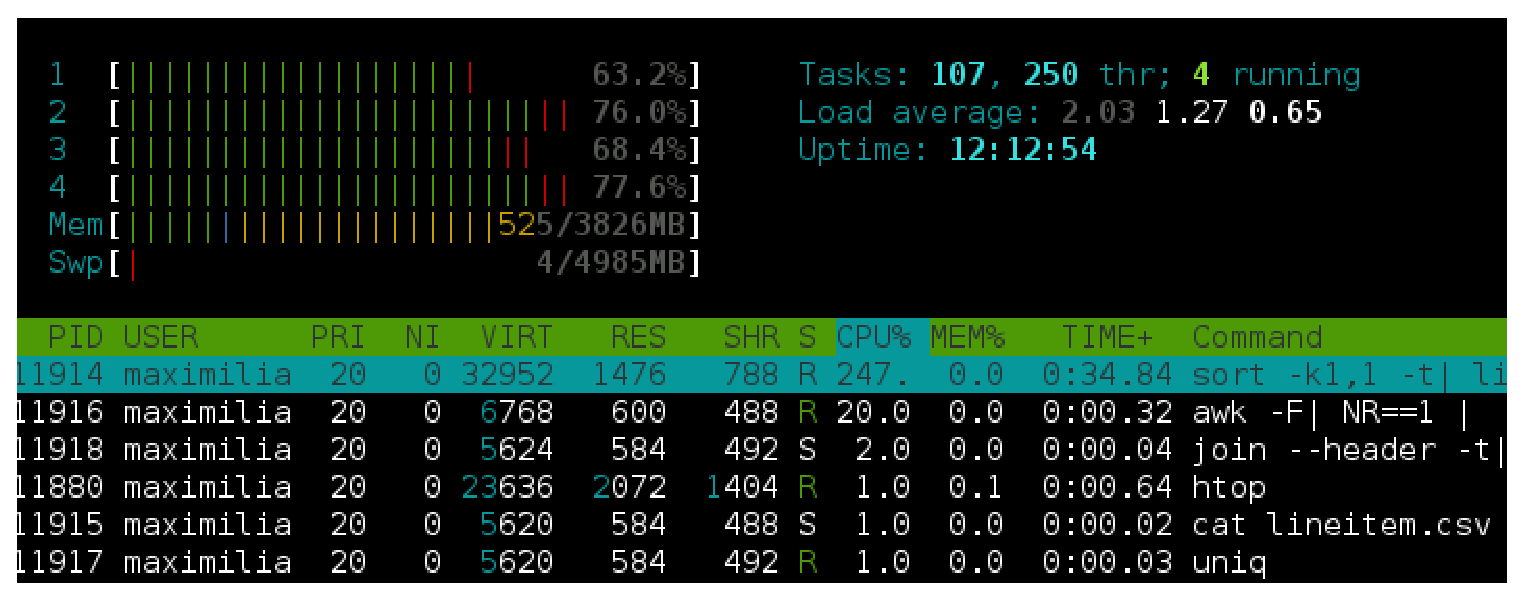
\includegraphics[scale=.5]{htop.eps}
\caption{Parallele Ausführung mittels Pipe verbundener Prozesse}
\label{fig:htop}
\end{figure}

\begin{quote}
"`Die Programme in der Pipeline werden in Wirklichkeit gleichzeitig ausgeführt, nicht nacheinander. Das bedeutet, da[ss] die Programme in einer Pipeline interaktiv arbeiten können; der Betriebssystem-Kern sorgt für die nötige Zuteilung von Rechenzeit und Synchronisation, damit alles funktioniert."' \cite[S. 34]{TUPE}
\end{quote}

Das Ziel ist es also, eine möglichst hohe Druchlaufquote durch die Verwendung von Pipelines zu erzielen. Jedoch geht dies nur bis zu einem gewissen Grad, die zwangsweise Sortierung der Datenbestände vor Joins macht die Aufteilung in einen Kopf und einen Rumpf erforderlich, der Kopf bleibt unverändert, der Rumpf wird sortiert und alles in eine Datei umgeleitet oder mit \textit{cat} wieder zusammengefügt.

\begin{lstlisting}[language=Bash]
head -1   tmprns.csv > tmp1.csv
tail -n+2 tmprns.csv | sort -t\| -k2,2 >> tmp1.csv
head -1   join5.csv > tmp2.csv
tail -n+2 join5.csv | sort -t\| -k2,2 | cat tmp2.csv - |\
join --header -t\| -1 2 -2 2 tmp1.csv - |\
\end{lstlisting}

Versuche, die Kommandos in eine Pipeline zu packen, schlagen kläglich fehl. Jetzt wäre es doch praktisch, ein alternatives Konstrukt zu nutzen, sodass die Verarbeitung parallel ablaufen kann. Benannte Pipes sind die Lösung, sie können einfach erstellt werden.

\begin{lstlisting}[language=Bash]
$ mkfifo mypipe
\end{lstlisting}

Wichtig ist, dass die Prozesse, die in die Pipe hineinschreiben und aus ihr herauslesen, parallel ablaufen. Die Pipe blockiert so lange, bis aus ihr gelesen, bzw. in sie geschrieben worden ist.

Nachfolgend ein einfaches Beispiel, das bereits 13\% Zeit einspart und zeitlich fast an eine Pipeline herankommt.\\
\lstinline{$ sort orders.tbl | grep final} benötigt 2,752 s\\
Ohne die Pipeline können die Prozesse über eine Datei kommunizieren oder über eine benannte Pipe:\\

{\footnotesize \texttt{ \parbox{7cm}{
%\begin{lstlisting}[language=Bash]
\#!/bin/bash\\
sort \$1 > tmpfile\\
grep final < tmpfile\\
%\end{lstlisting}
}
\parbox{7cm}{
%\begin{lstlisting}[language=Bash]
\#!/bin/bash\\
mkfifo mypipe\\
(sort \$1 > mypipe)\&\\
grep final < mypipe
%\end{lstlisting}
}}}\\


Mit Umlenkung in eine Datei werden 3,165 s gebraucht, die zweite Variante schlägt die erste mit nur 2,760 s und liegt damit dicht an einer Pipeline.
%real	0m2.752s
%user	0m7.620s
%sys	0m0.212s
%real	0m2.760s
%user	0m7.644s
%sys	0m0.212s
%real	0m3.165s
%user	0m7.488s
%sys	0m0.288s
Darüberhinaus ist es von Vorteil, dass ein Prozess im Hintergrund und somit auch parallel läuft. Und synchronisiert sind sie auch, sie müssen nicht explizit auf ihren Vorgängerprozess warten. Solange in die Pipe noch nicht geschrieben ist, wird der andere Prozess blockiert. Lediglich die Reihenfolge ist wichtig. Auf diese Weise werden die TPC-H-Anfragen nun optimiert: Zuerst wird die Kopfzeile geschrieben, dann der Rumpf.
\begin{lstlisting}[language=Bash]
head -1   tmprns.csv > tmp.csv &
tail -n+2 tmprns.csv | sort -t\| -k2,2 | cat tmp.csv - > tmp1.csv &
head -1   join5.csv > tmp2.csv &
tail -n+2 join5.csv | sort -t\| -k2,2 | cat tmp2.csv - |\
join --header -t\| -1 2 -2 2 tmp1.csv -
\end{lstlisting}

Analog dazu werden nun alle Anfragen optimiert und die neue Zeit gemessen.

\begin{tikzpicture}
\begin{axis}[
xtick=data,
legend style={at={(0.5,0.97)},
         anchor=north,legend columns=-1},
title=Abfragedauer bei SF1,
ybar = 0.25pt,
width=0.95\textwidth,height=0.48\textheight,
bar width=6pt,
xlabel={$Abfrage Nr.$},
ylabel={$Zeit [s]$},
]
\addplot[
ybar,
fill = blue,
] coordinates {
(1,47.420)
(2,6.372)
(3,32.022)
(4,22.544)
(5,26.827)
(6,7.949)
(7,18.713)
(8,39.677)
(9,54.243)
(10,12.971)
(11,2.934)
(12,22.859)
(13,7.068)
(14,7.185)
(15,29.784)
(16,4.957)
(17,37.156)
(18,25.484)
(19,6.728)
(20,58.405)
(21,63.225)
(22,6.178)
};
\addplot[
ybar,
fill=orange,
] coordinates{
(2,5.974)
(3,31.000)
(4,22.466)
(5,24.696)
(7,18.294)
(8,37.294)
(9,52.910)
(10,12.374)
(11,2.906)
(12,21.855)
(13,6.271)
(14,6.767)
(15,29.505)
(16,4.354)
(17,37.317)
(18,24.947)
(19,6.443)
(20,59.412)
(21,46.289)
(22,5.921)
};
\legend{original,optimiert}
\end{axis}
\end{tikzpicture}

\begin{tikzpicture}
\begin{axis}[
xtick=data,
legend style={at={(0.5,0.97)},
         anchor=north,legend columns=-1},
title=Abfragedauer bei SF10,
width=0.95\textwidth,height=0.48\textheight,
ybar = 0.25pt,
bar width=6pt,
xlabel={$Abfrage Nr.$},
ylabel={$Zeit [s]$},
]
\addplot[
ybar,
fill = blue,
] coordinates {
(1,	572.857)
(2,	73.534)
(3,	443.247)
(4,	234.677)
(4,	238.975)
(5,	307.112)
(6,	140.614)
(7,	260.438)
(8,	518.944)
(9,	304.204)
(10,	195.974)
(11,	34.194)
(12,	261.685)
(13,	100.206)
(14,	128.932)
(15,	446.731)
(16,	66.396)
(17,	468.63)
(18,	320.389)
(19,	175.907)
(20,	806.291)
(21,	891.314)
(22,	82.748)
};

\addplot[
ybar,
fill = orange,
] coordinates{
(2,	73.534)
(3,	443.247)
(5,	305.788)
(7,	254.706)
(8,	492.842)
(9,	277.647)
(10,	189.187)
(11,	34.22)
(12,	222.58)
(13,	90.957)
(14,	122.453)
(16,	56.808)
(17,	472.637)
(18,	308.145)
(19,	172.96)
(20,	812.589)
(21,	642.894)
(22,	77.706)
};
\legend{original,optimiert}
\end{axis}
\end{tikzpicture}

Bei fast allen Abfragen konnten leichte Verbesserungen erzielt werden, bei den meisten zwar nur unerheblich, aber bei der vorletzten Abfrage ist deutlich zu sehen, was ein bisschen Parallelisierung bewirkt, sie läuft um 28\ \% schneller.
Eine weitere Möglichkeit Parallelität zu erreichen ist die Prozesse mit \textit{split} aufzuteilen. Dieser Befehl erzeugt aus einer Datei mehrere kleine aufsteigend benannte Dateien (beginnend bei \textit{aa} bis \textit{zz}, auch mit benannten Pipes kompatibel), auf denen die Anfragen laufen. Das Zusammenfügen passiert am Ende mit \textit{cat}. Bei kleinen Anfragen dauert das Teilen länger als was die Parallelität einspart.

\begin{lstlisting}[language=Bash]
$ grep final lineitem.tbl
\end{lstlisting}
Das Skript nun mit geteilter Quelldatei und Ausführung der Prozesse im Hintergrund.
\begin{lstlisting}[language=Bash]
#!/bin/bash
mkfifo mini.aa mini.ab g1 g2
(split -n2 lineitem.tbl mini.)&
(grep final mini.aa > g1)&
(grep final mini.ab > g2)&
cat g1 g2

rm mini* g1 g2
\end{lstlisting}
Das Skript verdeutlicht die Parallelität durch Teilen, die getestete Ausführung benötigt jedoch 0,2\ s länger (2,8\ s statt 2,6\ s).\\

Komplizierter wird die Syntax, wenn die Parallelisierung über GNU Parallel läuft. Dieses bietet zahlreiche Funktionen an, die aber über den Inhalt dieses Kapitels - einfache Skripte wie sie in der Wissenschaft vorkommen zu erstellen - hinaus gehen. Zusammen mit nachfolgendem Beispiel sei aber auf die Literatur verwiesen \cite{DataScience}.
\begin{lstlisting}[language=Bash]
$ seq 4 | parallel "echo {}"
1
2
3
4
\end{lstlisting}
